\section{Evaluation}


\begin{table}[t!]
\centering
\caption{Result on \swebench{} Verified}
\label{tab:verified}
\scalebox{1}{
\begin{tabular}{ll|rr}
\toprule
 Tool & \llm & {\%{} Resolved} & {Avg. \$ Cost}\\
\midrule
 & \openai{} \gptfivemini{} & 59.8\% & \$0.04 \\
 & \openai{} \gptfive{} & 65.0\% & \$0.28 \\
 & \anthropic{} \claudesonnetfourfive{} & 70.6\% & \$0.56 \\
 \multirow{-4}*{\minisweagent{}~\citep{yang2024sweagent}} & \gemini{} \geminithreepro{} & 74.2\% & \$0.46 \\
\midrule
 & \openai{} \gptfivemini{} & 63.0\% & \$0.05 \\
 & \openai{} \gptfive{} & 68.4\% & \$0.27 \\
 & \anthropic{} \claudesonnetfourfive{} & 75.4\% & \$0.68 \\
\multirow{-4}*{\textbf{\tech{}}} & \gemini{} \geminithreepro{} & 77.4\% & \$0.48 \\
\bottomrule
\end{tabular}
}
\end{table}

\begin{table}[t!]
\centering
\caption{Result on \swebench{} Verified-60{}}
\label{tab:verified_subset}
\scalebox{1}{
\begin{tabular}{lll|rr}
\toprule
& Tool & \llm & {\%{} Resolved} & {Offline cost (hours)}\\
\midrule
\multirow{3}{*}{\rotatebox[origin=c]{90}{\makecell{\footnotesize{}Offline self-\\improving\\agents}}} & \sica{}~\citep{robeyns2025sica} & \openai{} \gptfivemini{} & 50.0\% & infinite loop \\
\cmidrule{2-5}
& \dgm{}~\citep{zhang2025darwin} & \openai{} \gptfivemini{} & 53.3\% & 1231 \\
\cmidrule{2-5}
& \hgm{}~\citep{wang2025huxley} & \openai{} \gptfivemini{} & 56.7\% & 512 \\
\midrule
\midrule
& {\textbf{\tech{}}} & \openai{} \gptfivemini{} & 65.0\% & 0 \\
\bottomrule
\end{tabular}
}
\end{table}


\subsection{Main Results}

\parabf{\swebench{} Verified.} 
Table~\ref{tab:verified} shows the results of \tech and prior agent approaches on \swebench Verified. 
We first observe that compared with \minisweagent{}, across four different \llm backends, \tech consistently achieves a higher resolve rate.
This demonstrates the improvement in performance enabled by allowing agents to create and use their own custom tools on the fly.
Furthermore, \tech is able to achieve this with only a minimal increase in cost compared with the base \minisweagent.
In certain cases (e.g., in \gptfive{}), we even observed slight cost savings where the agent can improve the solving efficiency by replacing complex, multi-turn commands with customs tools that achieve the same functionality.


We also demonstrate the comparison between \tech and the best-performing agentic tools, including both state-of-the-art open-source solutions and proprietary commercial scaffolds, on \swebench Verified (Figure~\ref{fig:result}).
We only report single-attempt results in Figure~\ref{fig:result} without any test-time scaling to ensure a fair comparison.
We observe that \tech using \geminithreepro{} achieves \textbf{a solve rate of 77.4\% without test-time scaling, outperforming all existing agents on the \swebench Verified leaderboard}\footnote{\url{https://www.swebench.com}} including state-of-the-art commercial solutions at the time of writing.

Furthermore, we perform a detailed comparison with three prior self-evolving agents on a subset of 60 \swebench Verified problems chosen by prior evaluation~\citep{wang2025huxley}.
Table~\ref{tab:verified_subset} shows the resolve rate and the offline cost for \sica, \dgm, \hgm, and \tech on the subset of problems.
We observe that \tech achieves the best performance, improving the resolve rate by 8.3 percentage points compared to previous best approach.
We also see that previous self-evolving agents all require a heavy amount of offline training to evolve the base agent, costing more than 500 hours.
Furthermore, prior self-evolving techniques produce a static agent used for all problems.
On the other hand, \tech creates customs tools for each individual task, allowing it to adapt on the fly based on the problem and specific LLM used.
Unlike the costly offline updates required by prior self-evolving agents, \tech instead adopts an online evolving approach to prompt the agent to generate custom tools on the fly to improve performance with minimal overhead.

\begin{table}[t!]
\centering
\caption{Result on \swebenchpro{}}
\label{tab:pro}
\scalebox{1}{
\begin{tabular}{ll|rr}
\toprule
 Tool & \llm & {\%{} Resolved} & {Avg. \$ Cost}\\
\midrule
\sweagent{}~\citep{yang2024sweagent} & \anthropic{} \claudesonnetfourfive{} & 43.6\% & - \\
\midrule
\textbf{\tech{}} & \anthropic{} \claudesonnetfourfive{} & 45.8\% & \$0.73 \\
\bottomrule
\end{tabular}
}
\end{table}

\parabf{\swebenchpro{}.} 
We also evaluate \tech on the public set of \swebenchpro, containing 731 problems across 11 repositories and four programming languages (Python, Go, TypeScript, and JavaScript).
Table~\ref{tab:pro} shows the performance of \tech compared to the state-of-the-art baseline of \sweagent on \swebenchpro~\cite{deng2025swe}.
Different from \minisweagent, which only has access to basic bash commands, \sweagent provides handcrafted file viewing and editing tools and is the best performing approach on the \swebenchpro.
We choose \claudesonnetfourfive{} for \sweagent because it ranks at the top of \swebenchpro leaderboard\footnote{\url{https://scale.com/leaderboard/swe_bench_pro_public}}, as such, we also use it as the base \llm for \tech to enable a fair comparison.
We observe that \tech is able to achieve better performance compared with \sweagent, a specially designed agent implemented with close to 7,000 lines of code.
We also compare with all other top-performing agents and \llm{s} in Figure~\ref{fig:result} and observe that \tech is able to achieve the \textbf{new state-of-the-art performance of 45.8\% resolve rate on \swebenchpro}.
This further demonstrates the superiority of the live scaffold design of \tech compared to existing agents that interact with a fixed set of manually-crafted tools.

\subsection{Tools Analysis}
\label{sec:tool_analysis}

\begin{figure*}[h]
    \centering
    \begin{subfigure}[b]{0.32\textwidth}
    \centering
    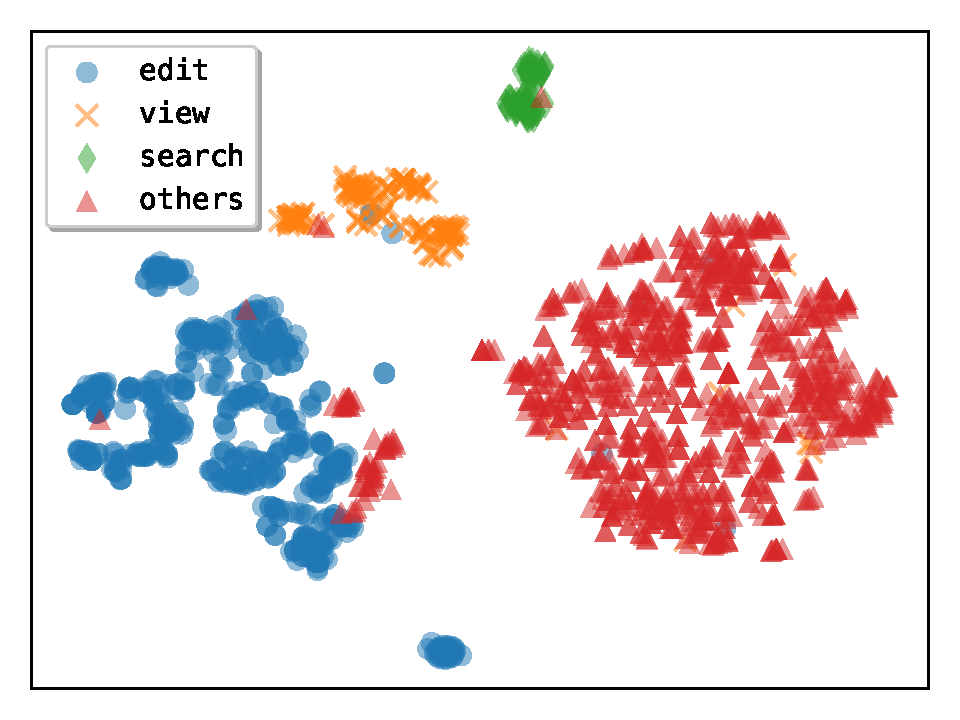
\includegraphics[width=\textwidth]{figs/tsne_verified_claude_tool_use.pdf}
    \caption{Tools in \swebench Verified}
    \label{fig:tool_verified}
\end{subfigure}
\begin{subfigure}[b]{0.32\textwidth}
    \centering
    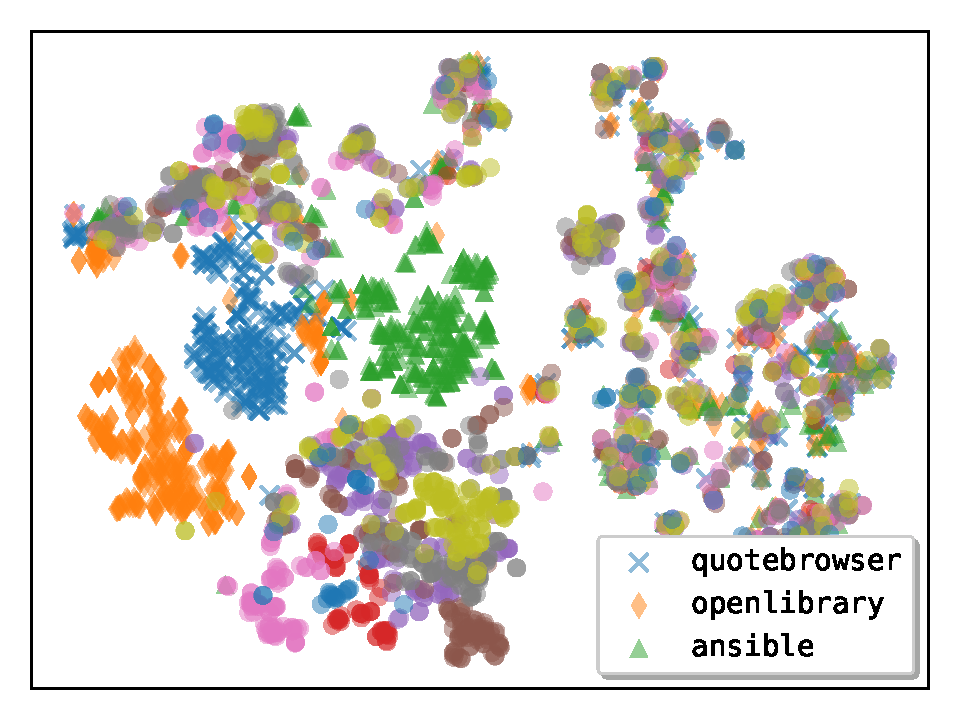
\includegraphics[width=\textwidth]{figs/tsne_verified_claude_pro.pdf}
    \caption{Tools in \swebenchpro{}}
    \label{fig:tool_pro_repo}
\end{subfigure}
\begin{subfigure}[b]{0.32\textwidth}
    \centering
    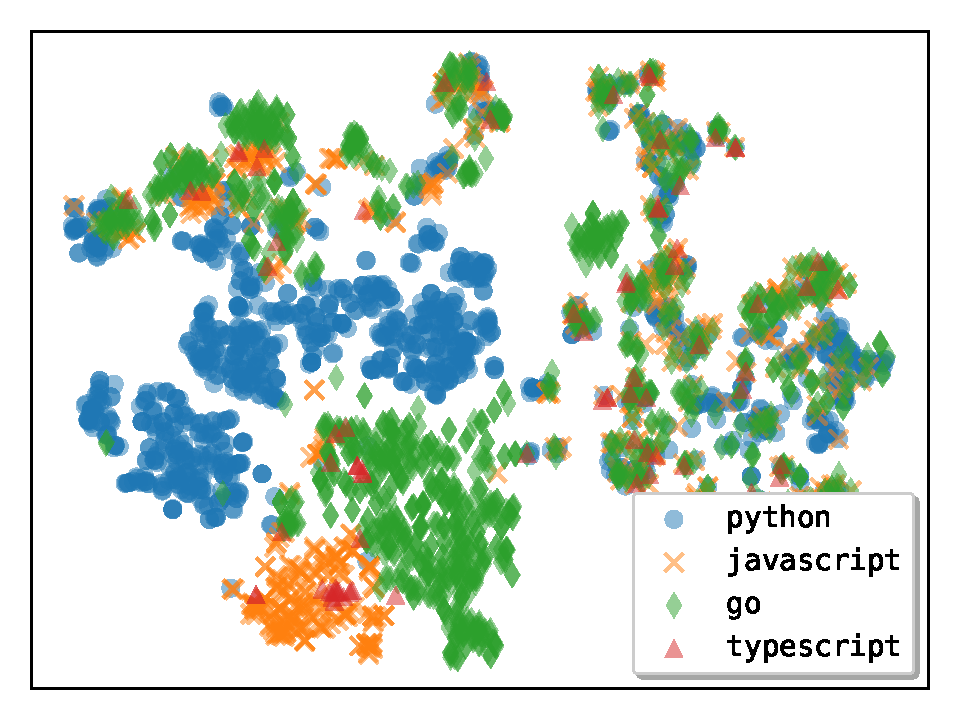
\includegraphics[width=\textwidth]{figs/tsne_verified_claude_pro_language.pdf}
    \caption{Tools in \swebenchpro{}}
    \label{fig:tool_pro_language}
\end{subfigure}
\caption{
2 dimensional t-SNE visualization of tools generated by \claudesonnetfourfive{} on \swebench Verified and \swebenchpro.
We label and display the embedding based on tool type (Figure~\ref{fig:tool_verified}), repository name (Figure~\ref{fig:tool_pro_repo}), and programming language used in the repository (Figure~\ref{fig:tool_pro_language}).
Note that for Figure~\ref{fig:tool_pro_repo}, we only label three repositories in the legend due to space considerations. 
The three repositories were chosen as they have representative distinct clusters.
}

\label{fig:tsne}
\end{figure*}

\parabf{Categories and variations of custom tools.}
We examine the custom tools created by \tech{}. 
Figure~\ref{fig:tsne} shows the embedding visualizations using t-SNE~\citep{hinton2002stochastic} of the tools created by \tech{}. 
We compute the embedding for each tool based on the tool body (i.e., the content of the tool script) using a text embedding model (OpenAI \CodeIn{text-embedding-3-small}).
To start off, we look at the types of tools created by \tech by categorizing them into common tool functionalities (e.g., edit, view, search, etc). 
We perform this categorization by using simple string matching based on the script filename of the tool.
Figure~\ref{fig:tool_verified} shows the visualization of the tools generated for \swebench Verified. 
We see that while there are definitely distinct clusters of common tools like edit, view, and search, there are still variations among them.
For example, the edit tool cluster (highlighted in blue circles) is not a tightly concentrated dot, but instead is spreadout, showing that \tech can generate different editing tools depending on the problem.
Furthermore, \tech also allows the agent to generate additional tools (the others category highlighted in red triangles). 
These are the more unique issue-specific tools such as a script that applies a very detailed patch to multiple files or a diff checking tool that shows the difference between two files.
We also apply similar analysis to all studied datasets in Appendix~\ref{appendix:tool_analysis}.


In addition to the types of tools created, we also examine how the tools created can change across different repositories and languages.
Figure~\ref{fig:tool_pro_repo} shows the visualization of the tools created in \swebenchpro categorized based on repositories.
In \swebenchpro, there are 11 different repositories, and not surprisingly, there are common tools created across different repositories (i.e., the overlapping clusters in the figure). 
On the other hand, there are also specific tools for certain repositories, for example we see a distinct cluster (highlighted in orange diamonds) for \CodeIn{openlibrary}, a codebase for cataloging literature.
Since \CodeIn{openlibrary} deals with lots of raw data of a specialized format, the custom tools generated by \tech are specifically tailored for that.
We also observe similar results when we break down the tools based on programming language of the repositories in Figure~\ref{fig:tool_pro_language}.
Different problems, environments, and languages may require completely different specialized tools, highlighting again how using the same set of tools for all problems is suboptimal.

\begin{wrapfigure}{r}{0.4\textwidth}
  \begin{minipage}{\linewidth}
  \centering
  \captionsetup[subfigure]{justification=centering}
  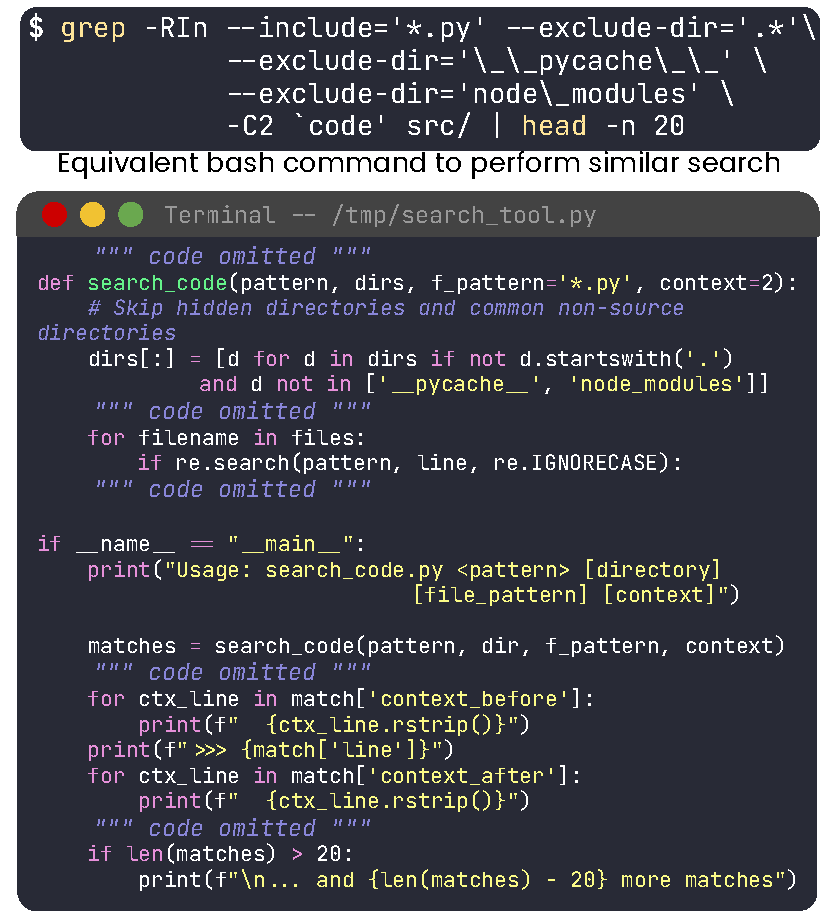
\includegraphics[width=\linewidth]{figs/example_tools_3.pdf}
  \subcaption{Search tool}
  \label{fig:example_tools3}
  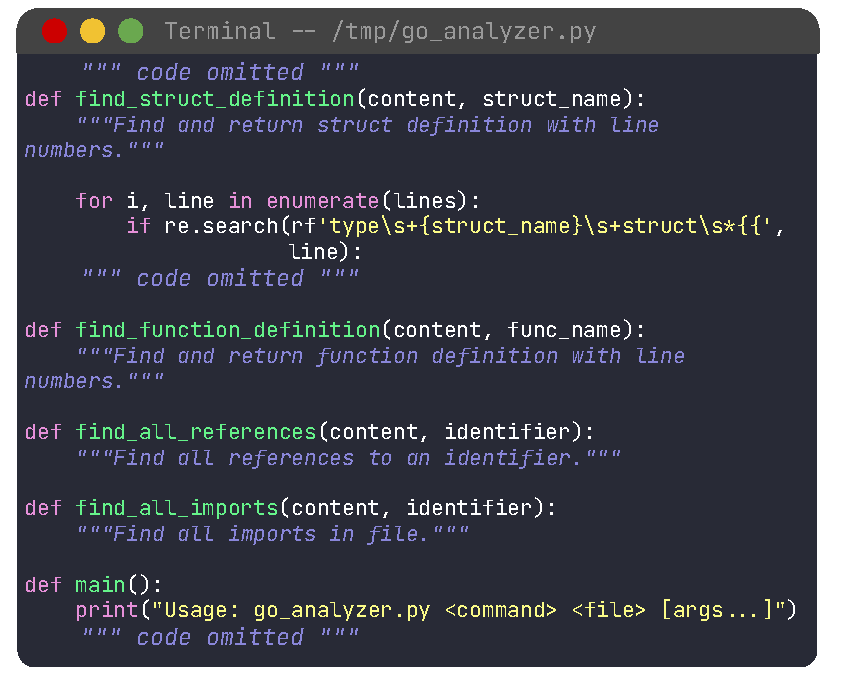
\includegraphics[width=\linewidth]{figs/example_tools_4.pdf}
  \subcaption{Go file analyzer tool}
  \label{fig:example_tools4}
  \end{minipage}
  \caption{Example custom tools}
  \label{fig:example_tools_big_2}
\end{wrapfigure}

\parabf{Effective and interesting custom tools.}
We now take a closer look at a few exemplary effective and interesting tools created by \tech.
Figure~\ref{fig:example_tools3} shows a custom search tool created by \tech.
This example might appear simple and straightforward at first glance.
However, it implements several important features: (1) supports focused searching within directories and pattern-based matching, (2) ignores irrelevant folders (\CodeIn{\_\_pycache\_\_} and \CodeIn{node\_modules}) and hidden folders (\CodeIn{.git}) during search, (3) displays relevant code context before and after the found code, and (4) limits results to top 20 matches to reduce context size.
By baking in the exclusion of irrelevant folders in the search tool, agents do not have to add these folders as a separate flag during the searching process.
Showing the relevant surrounding context is also helpful since oftentimes we want to find out how the code snippet of interest is being used.
Furthermore, only showing the first 20 matches can be critically important to not drastically inflate the context window, allowing the agent to easily refine their search to limit results.
An example bash command to emulate the functionality of the custom tool is shown at the top of Figure~\ref{fig:example_tools3}.
We can see the high degree of complexity in terms of options, arguments, and flags used in this long command.
On the other hand, we can simply call \CodeIn{"python search\_code.py `code' src/"} to perform the search via the custom tool.
By only using basic bash commands, the agent will have to chain together multiple commands using complex flags with potential to incur errors (e.g., older \CodeIn{grep} versions do not support features like \CodeIn{--exclude-dir}) or substantial slowdowns.
In fact, in our experimental results, we found that without access to custom tools, the agent may often take multiple steps to accomplish a basic task such as searching for relevant code.
This issue is further amplified when steps like search may need to be done multiple times for one task thus drastically limiting the problem solving efficiency and effectiveness.
By creating and introducing efficient and easy to use custom tools designed by agents themselves, \tech can improve agent performance on complex software engineering tasks.

Figure~\ref{fig:example_tools4} shows another custom tool \CodeIn{go\_analyzer.py} created by \tech. 
The tool can be used to analyze a Go file to find any struct and function definition, identifier references, and to obtain the imports used in the file.
This example showcases the powerful generative capability of agents where the custom tool can be used as a simple static analyzer for the Go programming language to search and provide key information about a file.
Different from the previous search tool example where one can technically mimic the behavior using bash commmands, abeit using very complex chain commands, the tool logic here is even more complex.
The custom tool performs strategic pattern matching based on Go grammar and provides an interface to support multiple different usages.
Furthermore, by saving this custom tool in an executable script, the agent can reuse the functionality multiple times.
By creating and using this custom tool to better understand file structure and content, \tech is able to solve this issue\footnote{\CodeIn{navidrome\_\_navidrome-10108c63c9b5bdf2966ffb3239bbfd89683e37b7}, \swebenchpro{}} that prior best performing baseline could not.

\subsection{Ablation}
\label{sec:ablation}

To evaluate the effect of different setups of \tech, we use a random subset of 50 problems in \swebench Verified (see Appendix~\ref{appendix:ablation_dataset} for the detailed list of problems).
Unless otherwise stated, we use \claudesonnetfourfive{} in our ablation experiments.

\begin{table}[t!]
\centering
\caption{Ablation result across \tech setups on subset of \swebench Verified problems}
\label{tab:ablation_setup}
\scalebox{1}{
\begin{tabular}{l|ll}
\toprule
 Approach & \% Resolved & \# of tools created\\
 \midrule
\tech{} w/o tool creation & 62.0\% & 0.00 \\
\tech{} w/o reflection & 64.0\% & 2.92 \\
\tech{} & 76.0\% & 3.28 \\
\bottomrule
\end{tabular}
}
\end{table}

\parabf{Effectiveness of tool creation steps.} 
Table~\ref{tab:ablation_setup} shows the impact of different components of \tech have on performance.
We see that by removing the on-the-fly tool creation ability of \tech (i.e., using the base \minisweagent), we achieve the lowest solve rate.
The performance is improved when we indicate to the agent to create custom tools in the initial prompt (row \tech w/o reflection).
However, the highest resolve rate is achieved once we explicitly ask the agent to reflect on the past trajectories to determine if they should create any tools after each step.
In our experiments, we found that this reflection process provides a good reminder for the agent to create tools that are specifically designed for the particular issue.
Furthermore, while the number of tools do not necessary correlate with solving performance, we also see that this reflection process creates more tools on average compared to only indicating the tool creation in the initial prompt. 
\tech is able to improve performance by reflecting on both the current problem and past trajectories to create custom tools on the fly.

\begin{table}[t!]
\centering
\caption{Ablation result across different \llm backends on subset of \swebench Verified problems}
\label{tab:ablation_llm}
\scalebox{1}{
\begin{tabular}{l|ll}
\toprule
 \llm & \minisweagent & \tech{}\\
 \midrule
\openai{} \gptfivenano{} & 44.0\% & 14.0\% \textcolor{red}{($\downarrow$-68.2\%)} \\
\openai{} \gptfivemini{} & 60.0\% & 58.0\% \textcolor{red}{($\downarrow$-3.3\%)} \\
\openai{} \gptfive{} & 60.0\% & 68.0\% \color[HTML]{009933}{($\uparrow$13.3\%)} \\
\midrule
\anthropic{} \claudesonnetthreeseven{} & 46.0\% & 50.0\% \color[HTML]{009933}{($\uparrow$8.7\%)} \\
\anthropic{} \claudesonnetfour{} & 58.0\% & 64.0\% \color[HTML]{009933}{($\uparrow$10.3\%)} \\
\anthropic{} \claudesonnetfourfive{} & 62.0\% & 76.0\% \color[HTML]{009933}{($\uparrow$22.6\%)} \\
\bottomrule
\end{tabular}
}
\end{table}

\parabf{Different \llm backends.} 
We now examine the effect of using different \llm backends for \tech.
Table~\ref{tab:ablation_llm} compares the performance of the base \minisweagent and \tech as we vary the \llm used on the same 50 problems used in the previous ablation experiment.
We first observe that there are weaker \llm{s} for which using \tech to create custom tools on the fly even decreases performance.
In particular, we see that for \gptfivenano{}, the results are significantly worse when using \tech compared to base \minisweagent.
After examining the trajectories, we found that \gptfivenano{} fails to understand the goal of creating custom tools and is often stuck in a loop thus leading to reduction in performance.
This indicates that weaker \llm{s} may lack the high-level reasoning capabilities to synthesize useful tools on the fly.
However, we see that \tech is able to improve more over the base \minisweagent as we start to use more powerful models.
Specifically, state-of-the-art \llm{s} such as \claudesonnetfour{} and \gptfive{} achieves the highest relative resolve rate improvement when using \tech compared with \minisweagent.
This demonstrates the generalizability of \tech across high-performing \llm{s} and the potential for \tech to further improve performance especially as we continue to build more and more powerful \llm{s}.

\begin{table}[t!]
\centering
\caption{Result on a subset of \swebenchmultilingual{} problems}
\label{tab:multilingual}
\scalebox{1}{
\begin{tabular}{ll|rr}
\toprule
 Tool & \llm & {\%{} Resolved} & {Avg. \$ Cost}\\
\midrule
\minisweagent{}~\citep{yang2024sweagent} & \anthropic{} \claudesonnetfourfive{} & 40.0\% & \$0.59 \\
\midrule
\textbf{\tech{}} & \anthropic{} \claudesonnetfourfive{} & 46.0\% & \$0.66\\
\bottomrule
\end{tabular}
}
\end{table}


\parabf{\swebenchmultilingual{}.} 
In addition to evaluating on \swebench Verified and \swebenchpro, we also test the generalizability of \tech on other benchmarks. 
We conducted an initial experiment on a subset of 50 problems (see Appendix~\ref{appendix:multilingal_subset} for the detailed list of problems) in \swebenchmultilingual~\citep{sbm}, a benchmark of software engineering tasks across 9 programming languages (JavaScript, TypeScript, Rust, Ruby, Go, C/C++, PHP, and Java).
\Cref{tab:multilingual} shows the performance of \tech compared to \minisweagent on \swebenchmultilingual. 
We observed that \tech achieves a better performance by obtaining a resolve rate of 46.0\%, while \minisweagent only has a resolve rate of 40.0\%.
This demonstrates the generalizability of \tech on additional challenging problems.

\subsection{Discussion and Future Work}

\parabf{Towards general, on the fly self-evolution.}
In this work, \tech primarily focuses on enabling agents to self-evolve through custom tool creation and usage.
As discussed previously, the key idea of \tech, to improve and modify the agent itself on the fly, extends beyond creating new tools to also modifying the entire agent implementation.
This includes the overall system prompt of the agent, how the agent interacts with the environment, and even the concrete workflow of the agent when it attempts to solve the issue.
We believe that the entire agentic loop, much like any other software, can be modified and improved especially on the fly based on feedback and insights gained from solving a problem.
Furthermore, we hope to extend the self-evolution loop across different tasks as well.
Instead of discarding each evolved agent after a task is completed, we can save and
serialize the useful tools and insights (via concepts like Skills~\cite{skills}) for future tasks.
The agent can then load these useful tools and insights obtained while solving previous tasks on the fly  
to further improve performance and support continuous self-evolution across tasks.

\parabf{Impact on \llm evaluation.}
Our experimental results on multiple benchmarks using multiple \llm{s} demonstrate that \tech can achieve state-of-the-art performance.
This shows that \tech can provide an effective scaffold for unified evaluation of \llm performance on solving software development issues.
Instead of using complex or proprietary agent scaffolds, \tech provides a simplistic and lightweight approach that can be easily added on top of any agent design to evaluate \llm{s}. 
Moreover, \tech not only evaluates the issue solving ability, but it can also test the tool-creation capability of \llm{s} and agents.
Tools are one of the most important aspect of an agent and directly impacts the issue solving performance.
The ability for \llm{s} to create custom tools, especially for solving complex software development issues, have not been extensively evaluated.
To this end, we have already seen some interesting results in our evaluation where weaker \llm{s} lack high-level reasoning to create useful tools on the fly (see Section~\ref{sec:ablation}).
\tech provides a unique framework to jointly evaluate both the tool creation and issue resolution ability of \llm{s}.

\parabf{Applications beyond software issue resolution tasks.}
In addition to software issue resolution tasks, \tech can be easily applied to other challenging software engineering tasks like generating tests~\cite{deng2023large}, detecting and patching vulnerabilities~\cite{lee2025sec}, and synthesizing production-ready software from scratch~\cite{zhao2024commit0}.
Compared with issue resolution tasks, other software problem domains will require even more task-specific and diverse tools and agent scaffolds.
For example, to detect malicious vulnerabilities in commercial off-the-shelf binaries, we need binary analysis tools and decompilers. 
To optimize a large complex system, we need to apply profilers and tracing tools.
Instead of using a fixed agent scaffold with basic tools that cannot adopt to different problem domains or painstakingly designing specialized agents for each individual task, \tech can easily generalize to solving tasks in different domains by automatically modifying itself on the fly based on the task at hand.

\parabf{Self-evolution during \llm training.}
In this work, \tech is implemented as a lightweight modification to an existing agent, requiring no offline training or updates.
However, the idea of on-the-fly self-evolution can also be easily extended to \llm training, where instead of learning from a fixed workflow and a static set of tools, the \llm learns to also create new tools and modify the scaffold itself during training. 
In this approach, the resulting \llm will have improved reasoning capabilities as the self-evolving training approach provides additional learning signals, allowing the \llm to solve more complex tasks. 
Through self-evolving training, \llm{s} can learn to better create useful, task-specific tools and modify advanced scaffolds dynamically based on the problem at hand. 
Moreover, the final trained \llm will be compatible with more runtime agent frameworks since it is able to learn from its own created tools and modified scaffolds rather than relying on predefined scaffolds. 
This adaptability allows it to be more robust and generalize effectively to new scaffold setups and
even different tasks.

